
\documentclass[letterpaper,twocolumn,openany,nodeprecatedcode,dvipsnames,nomultitoc]{dndbook}
\usepackage[spanish]{babel} 
\usepackage[utf8]{inputenc}
\usepackage[singlelinecheck=false]{caption}
\usepackage{lipsum}
\usepackage{listings}
\usepackage{shortvrb}
\usepackage{graphicx}
\usepackage{etoolbox}
\usepackage{multicol}
\usepackage{url}
\usepackage{hyperref}
\usepackage{stfloats}
\usepackage{dirtytalk}
\usepackage{float}
\captionsetup[table]{labelformat=empty,font={sf,sc,bf,},skip=0pt}
\MakeShortVerb{|}
\lstset{%
basicstyle=\ttfamily,
language=[LaTeX]{TeX},
breaklines=true,
}
\begin{document}
\title{\huge APLICACIONES TELEMÁTICAS}
\author{

\includegraphics[width=6cm,height=6cm]{Manual/img/iconosinfondo.png} \\

\hspace{10pt}
Incredible Abroad Aider Application\vspace{10pt}\\
\textit{Andrés Ferrando Navarro}\\
\textit{Àlex Ganau Sánchez}\\
\textit{Alejandro Gómez Gambín}\\
\textit{Iván Ibáñez Zamora}
}

\date{22/06/2020}

%--------------------------------%
%--------------------------------%

\frontmatter
\maketitle
\tableofcontents

\mainmatter
\part{Sketches}
\vspace{10pt}
\section{INTRODUCCIÓN}
\vspace{5pt}

\begin{justify}

\DndDropCapLine{E}l presente documento recoge el manual con el funcionamiento de la aplicación diseñada para el proyecto final de la asignatura \textit{Aplicaciones Telemáticas}.

\end{justify}

\par 
\begin{justify}

Esta sección incluye los bocetos iniciales de la UI (User Interface) de la App así como algunos comentarios sobre los cambios durante el desarrollo de la misma.


\section{SKETCHES}

\vspace{5pt}

Antes de ponerse a trabajar en Android Studio, un desarrollador debe tener claro el aspecto que va a tener su aplicación. Para ello, se utilizó la web \textbf{NinjaMock} que permite hacer bocetos de aplicaciones de forma rápida y sencilla. Además, llama mucho la atención el estilo visual que tiene, como si estuvieran hechos a mano.

\subsection{Pantalla de Inicio}
\begin{figure}[h]
\centering
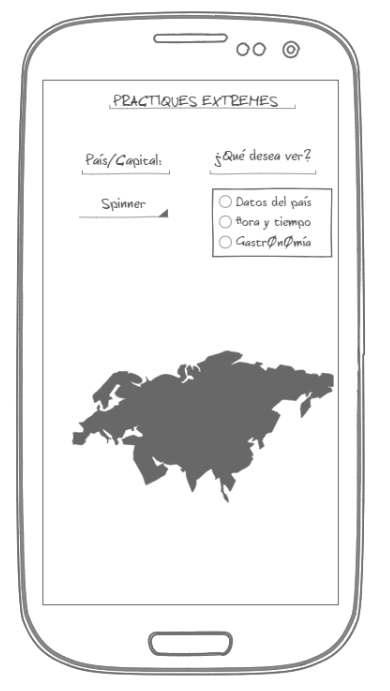
\includegraphics[scale = 0.2]{Manual/img/Pantalla Main.png}
\end{figure}

En versiones posteriores, al añadir otras clases que usaran mapas, se sustituyó este por un GIF de la bandera de la Unión Europea
\subsection{Datos del País}
\begin{figure}[h]
\centering
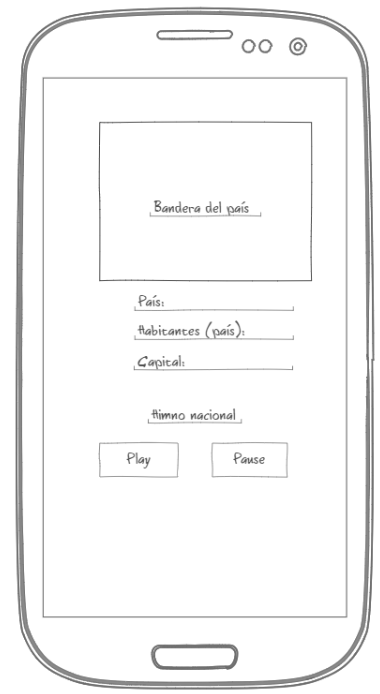
\includegraphics[scale = 0.2]{Manual/img/Datos Pais.png}
\end{figure}
Posteriormente, se añadieron más datos relativos al país y los botones de Play y Pause se fusionaron en uno sólo que iba alternando entre ambas funciones según estuviera sonando el himno o no.
\subsection{Hora Y Tiempo}
\begin{figure}[H]
\centering
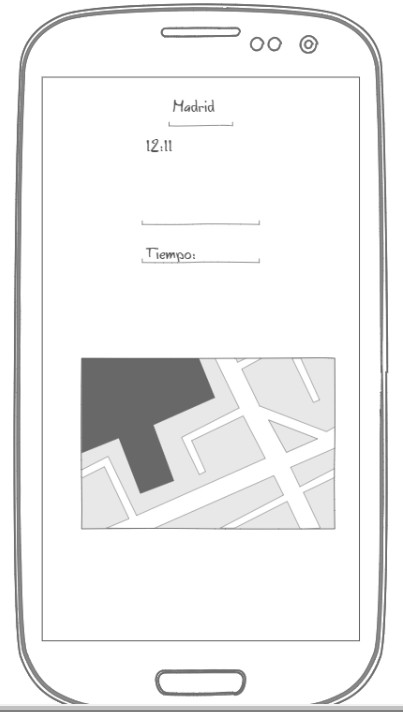
\includegraphics[scale = 0.2]{Manual/img/Hora Y Tiempo.png}
\end{figure}
\subsection{Gastronomia}
\begin{figure}[H]
\centering
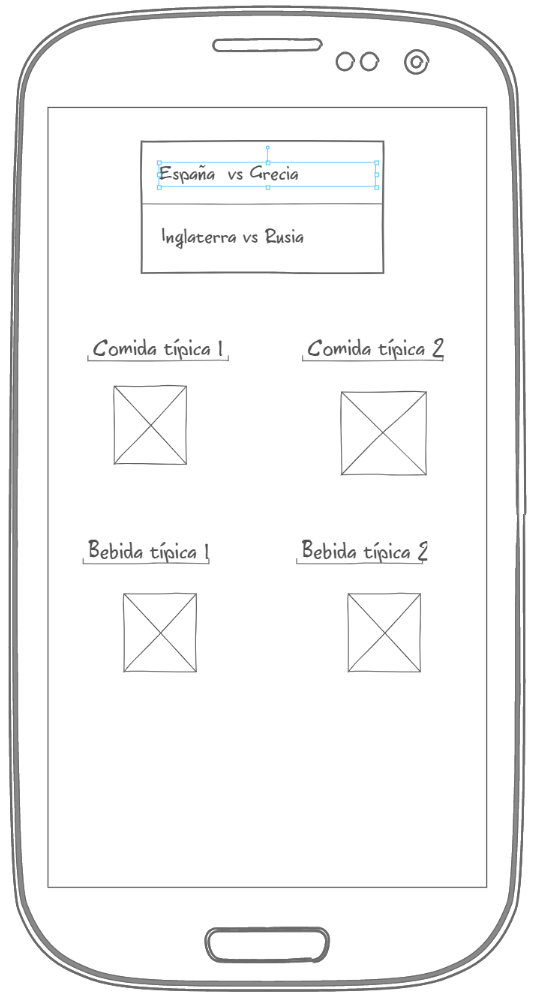
\includegraphics[scale = 0.3]{Manual/img/Pantalla Gastronomia.png}
\end{figure}
Se ha tenido en cuenta que en España hay más comidas que en otros países por lo que la interfaz variará de país a país.
\vspace{5pt}
\section{DESARROLLO}
\vspace{3pt}
En versiones posteriores de la app, se añadieron dos actividades nuevas para poder hacer uso de más funcionalidades de Android Studio tales como las librerías Glide para mostrar Gifs, las bases de datos en tiempo real Firebase y mostrar un mapa en pantalla completa con marcadores personalizados y vista satélite. Estas dos actividades no tienen sketches ya que no estaban previstas en el plan inicial de desarrollo.

\begin{DndReadAloud}
  \textbf{NOTA: }Esta aplicación ha sido adaptada para el terminal Google Nexus 5 con la API 29 con una pantalla de, aproximadamente, 5 pulgadas.
\end{DndReadAloud}

\end{justify}

\part{Funcionamiento}
\vspace{10pt}
\section{INTRODUCCIÓN}
\vspace{5pt}

\begin{justify}

\DndDropCapLine{E}n esta sección se incluyen las explicaciones necesarias para entender de una mejor manera cómo funciona la aplicación y todos sus componentes. 

\end{justify}

\par 
\begin{justify}

Además, se exponen brevemente las partes de código diseñadas mostrando los principales métodos utilizados para llevar a cabo cada una de las actividades que conforman la aplicación.

%--------------------------------%

\section{SPLASH SCREEN}

\vspace{5pt}

\par 
En primer lugar se encuentra la pantalla de bienvenida, la primera actividad de la aplicación, en la cual se muestran tanto los nombres de los integrantes del grupo como el icono de la aplicación, funcionando por tanto como una simple transición al main activity de la aplicación.

\vspace{5pt}

\par
Lo primero a tener en cuenta es especificar la splash screen en el \textit{AndroidManifest.xml} como actividad principal, ya que es la primera que se ejecuta, para así saltar al \textit{main activity}.

\vspace{5pt}

\par
La actividad se compone del método \textit{onCreate}, el cual se encarga de mostrar el layout \textit{activity\_splash\_activity.xml} compuesta por \textit{TextViews} y una \textit{ImageView}. Además, también se especifica la duración de la pantalla de bienvenida y ejecución del salto a \textcolor{RoyalBlue}{activityMain}.

%--------------------------------%

\section{PANTALLA DE INICIO}
\vspace{5pt}

\par 
La pantalla principal se encargará de hacer los saltos a las diferentes actividades que componen la aplicación, funcionando de la siguiente forma:

\par 
\begin{itemize}

    \item Relacionar los elementos del layout principal a las diferentes variables, como por ejemplo: \textit{Button \_btn = findViewById(R.id.\textcolor{purple}{btn})}.
    \vspace{5pt}
     
    \item Crear los adaptadores del spinner, un bundle, e introducir el gif mediante Glide (imágen desde una URL a un \textit{ImageView}).
    \vspace{5pt}
      
    \item Creación del método \textit{onClick} implementando la interfaz \textcolor{RoyalBlue}{View.OnClickListener} : se realiza un \textit{switch} dependiente de la información que se desee ver (Datos del país,gastronomía...), en el cual se crea un \textit{intent} y, según la opción escogida, se introducirá como parámetro el \textit{.class} de una actividad u otra. Dentro de cada case, se realiza otro \textit{switch}, el cual dependerá del país elegido en el que se introduce en el \textit{Bundle} la \textit{string} necesaria que utilizarán las diferentes actividades para mostrar la información elegida.
    \vspace{5pt}
    
    \item Lanzamiento de la actividad oportuna dependiente del \textit{Intent} creado.
    
\end{itemize}

\vspace{5pt}

\par
En esta pantalla se han utilizado \textit{TextViews}, un spinner, \textit{RadioButtons}, gifs y \textit{Buttons}. Además, se han implementado los saltos a diferentes actividades, usando los \textit{bundles} e \textit{intents} necesarios.

%--------------------------------%

\section{DATOS DEL PAÍS}
\vspace{5pt}
\subsection{FUNCIÓN}
\par 
Esta actividad se centra en mostrar los datos más importantes del país seleccionado. Para ello, en primer lugar aparece en la parte superior el nombre del país seleccionado por el usuario. Debajo de este aparece la bandera nacional del país, seguida de los siguientes datos técnicos:
\vspace{5pt}
\begin{center}
 POBLACIÓN CAPITAL GENTILICIO \par
 IDIOMA MONEDA HIMNO 
\end{center}
\vspace{5pt}
\par 
En la parte inferior de la pantalla, se puede apreciar un botón azul con el símbolo \textit{play} o \textit{pause}, según el momento, que permite escuchar el himno nacional de cada país.

\subsection{DESARROLLO DEL CÓDIGO}
\vspace{5pt}
\par
En primera instancia, antes de empezar a realizar el código de la actividad, se buscaron todas las imágenes de las banderas de los países y se descargaron los archivos \textit{.mp4} correspondientes a los himnos, guardando las imágenes en el directorio res/drawable y los audios en res/raw.
\vspace{5pt}
\par
A continuación se empezó a elaborar la clase llamada \textcolor{RoyalBlue}{datosPais}, la cual extiende a la clase \textcolor{RoyalBlue}{AppCompatActivity} e implementa la interfaz \textcolor{RoyalBlue}{View.OnClickListener} y cuyas variables declaradas son: 
\textit{Bundle b}, \textit{String pais}, \textit{MediaPlayer player} y \textit{Button reproductor}.
\vspace{5pt}
\par
Posteriormente, se realizó el método \textcolor{BurntOrange}{onCreate}, que consta de los siguientes aspectos:
\begin{enumerate}
    \item Llamada al constructor padre y la aplicación del layout.
    \item Extracción del país seleccionado a través del \textit{Bundle} creado.
    \item Definición del reproductor mediante \textit{setOnClickListener(this)}.
    \item Asignación de los \textit{ImageView} y \textit{TetxView} del layout.
    \item Un \textit{switch} que contiene los diferentes datos a mostrar en pantalla mediante \textit{Strings}, según el país seleccionado, así como la asignación al reproductor del himno que debería sonar del siguiente modo:
    \begin{DndSidebar}{Código para la reproducción del himno}
    \centering
    \par 
    \textit{player=MediaPlayer.create(this,R.raw.\textcolor{purple}{himno\_pais});}
    \end{DndSidebar}
\end{enumerate}
\vspace{5pt}
\par
Finalmente, se encuentran los métodos creados \textcolor{BurntOrange}{onClick}, cuyo cometido es, mediante el método de la clase \textcolor{RoyalBlue}{MediaPlayer} \textcolor{BurntOrange}{isPlaying()}, determinar si debe aparecer el botón de \textit{play} o \textit{pause}, según se esté o no reproduciendo el himno del país, y \textcolor{BurntOrange}{onBackPressed}, que tiene la función de detener el audio, en caso que el usuario utilice el botón \textit{back} para volver a la pantalla principal.

%--------------------------------%

\section{HORA Y TIEMPO}
\vspace{5pt}

\par 
La funcionalidad de esta pantalla es mostrar la hora y el tiempo atmosférico actuales en la capital del país seleccionado, aparte de un mapa de la capital en Google Maps.

\subsection{Obtención de la Hora}

El procedimiento para obtener la hora es exactamente el mismo que el seguido en la \textbf{Práctica 1} de Aplicaciones Telemáticas con la excepción de que ahora todo este proceso debe ejecutarse en un hilo paralelo al de la UI, es decir, se creó una clase que hereda de \textcolor{RoyalBlue}{AsyncTask} para pedir la hora en su método \textcolor{BurntOrange}{doInBackGround} y que actualice el reloj en \textcolor{BurntOrange}{onPostExecute}.

\begin{DndReadAloud}
\textbf{NOTA: }Esta vez, el servidor NTP utilizado es \textit{es.pool.ntp.org}
\end{DndReadAloud}
Además, como en la práctica misma, se ha incluido una clase llamada \textcolor{RoyalBlue}{Utiles} que incluye los métodos desarrollados para convertir un array de bytes a un Long, entre otros.

\vspace{3pt}
En cuanto al \textit{TextView} de la hora, se ha cambiado su tamaño y su fuente para que destaque por encima de todos los elementos de la pantalla.

\begin{DndTable}[header=Zonas Horarias]{XX}
    \textbf{Capitales}  & \textbf{Huso Horario} \\
     Londres - Lisboa & GMT \\
     París - Madrid & GMT + 1 \\
     Atenas - Moscú & GMT + 2 \\
\end{DndTable}

\subsection{Obtención del Tiempo}

Si bien en la \textbf{Práctica 2} de la asignatura se usaba la API REST para contactar con los servidores de AEMET, esta vez, como se necesita el tiempo en distintas zonas de Europa, se ha recurrido a la \textit{OpenWeather API}, una API Freemium que permite, en su versión gratuita realizar peticiones de tiempo atmosférico de cualquier zona del mundo con un límite de 100 peticiones por día. Para más información visitar \url{https://rapidapi.com/community/api/open-weather-map}
\vspace{3pt}

El paquete utilizado para hacer peticiones HTTP de forma sencilla es OKHTTP, disponible a través de los repositorios de Gradle:
\begin{DndSidebar}{Descarga del paquete OKHTTP}
\centering
\par \textit{implementation \textcolor{OliveGreen}{'com.squareup.okhttp:okhttp:2.5.0'}}
\end{DndSidebar}
    
La estructura para la petición de tiempo se detalla en la web adjunta y será constante en nuestro caso con la salvedad de la zona solicitada, que se codifica con un código de municipio con la siguiente estructura: \par \textit{Nombre de la ciudad,código de país}

Una vez obtenida la respuesta del servidor, ésta se pasa por el JSON Parser y se obtienen los datos y se hacen los cambios de unidades pertinentes. Por ejemplo, para la temperatura máxima:

\begingroup
\DndSetThemeColor[PhbMauve]
\begin{DndSidebar}{Ejemplo de lectura del JSON del tiempo}
\textit{int TempMax = raiz1.getJSONObject("main").getInt("temp\_max") - 273;}
\end{DndSidebar}
\endgroup

Cabe destacar que, al igual que se hará en la clase \textcolor{RoyalBlue}{GastronomiaActivity}, los TextView se harán invisibles en primera instancia con \textit{setVisibility(View.\textcolor{purple}{INVISIBLE})} hasta que se obtengan los datos. Cuando esto suceda, se harán visibles con \textit{setVisibility(View.\textcolor{purple}{VISIBLE})}.

Para finalizar esta subsección, hay que resaltar que se han usado las librerías Picasso que permiten, de una forma sencilla y breve, descargar una imagen de Internet y ponerla en un \textit{ImageView}. Esto se ha hecho para mostrar el estado del cielo de una forma gráfica, justo al lado de la hora. La instrucción empleada fue la siguiente, teniendo en cuenta que el JSON de la API ofrece un número que te permite descargarte el icono que muestra el estado del Cielo:

\begin{DndSidebar}{Descarga e Inserción de una imagen con Picasso}
\par \textit{ Picasso.get().load(\textcolor{OliveGreen}{http://openweathermap.org/img/wn/} + iconoCielo + \textcolor{OliveGreen}{@2x.png}).into(Cielo);}
\end{DndSidebar}

\subsection{Avance de la Hora}
Como añadido al plan inicial de desarrollo, se creó otra \textcolor{RoyalBlue}{AsyncTask} que creaba un hilo que se ejecutaba cada segundo para actualizar el reloj de la UI y asi producir su avance como si fuera un reloj real.
\vspace{3pt}

El algoritmo seguido para actualizar la hora se detalla en los comentarios del código correspondiente. La única parte reseñable es tener cuidado con hacer el \textit{setText} en el método \textcolor{BurntOrange}{onPostExecute} atendiendo a una serie de condiciones que hagan que siempre se muestren dos dígitos para cada magnitud del tiempo (horas, minutos y segundos). Por ejemplo si son las \textbf{17:03:54}, se debe mostrar el 0 que va a la izquierda del 3 en los minutos. Si se imprime el número directamente, esto no ocurre, sólo se mostraría el 3, de ahí la condición que se le ha impuesto al \textit{setText} en la línea 284 de la clase \textcolor{RoyalBlue}{avanzaTiempo}.
\vspace{3pt}

Las últimas instrucciones de \textcolor{BurntOrange}{onPostExecute} hacen que se cree una nueva Tarea Asíncrona del mismo tipo que se está ejecutando cíclicamente hasta que el usuario cierre esta actividad.

\subsection{Mapa de la capital}
Como último añadido, usando la API de Google Maps, se ha colocado un \textit{fragment} en el layout que se asocia a un \textit{SupportMapFragment} en el código de \textcolor{RoyalBlue}{horaYTiempo}. 

\vspace{3pt}
Cuando se ejecuta \textit{mapFragment.getMapAsync( \textcolor{orange}{this})} se llama al método \textcolor{BurntOrange}{onMapReady} en el cual, dependiendo del país elegido, se crea un objeto \textit{LatLng} con las coordenadas de la capital de país correspondiente y se mueve la cámara y se hace zoom sobre ella:

\begingroup
\DndSetThemeColor[PhbMauve]
\begin{DndSidebar}{Movimiento de la cámara y Zoom}
  \textit{googleMap.moveCamera(CameraUpdateFactory. newLatLngZoom(currentLocation,10));}
\end{DndSidebar}
\endgroup
Las posibilidades de los objetos \textit{GoogleMap} se extenderán un poco más en la sección de Embajadas.

%--------------------------------%

\section{GASTRONOMÍA}
\vspace{5pt}

\par 
Esta sección recoge el diseño y la realización de la gastronomía asociada a cada uno de los países escogidos. Para ello, se han incluido varios platos típicos y una bebida tradicional de cada país, de entre una gran variedad disponible para cada uno de ellos.

\vspace{5pt}

\par 
Respecto al funcionamiento, éste es muy simple debido a que sólo hay que seleccionar en la pantalla principal el país deseado y lo que se desea ver, en este caso, la gastronomía. Una vez en la actividad, aparecen, como bien se ha comentado antes, para el caso de Rusia, Grecia, Inglaterra, Francia y Portugal, una selección de dos de los platos típicos de cada territorio, así como una de sus bebidas típicas y tradicionales. 

\vspace{5pt}

\par 
Por otra parte, dado que nos encontramos en España y, a decir verdad, es uno de los países europeos que ofrece una de las mejores diversidades en referencia a los platos típicos del territorio español, se han escogido cuatro platos tradicionales y una bebida, aunque se podrían poner más de treinta exquisiteces según los distintos territorios que conforman nuestro país.

\vspace{5pt}

\par 
Cabe indicar que, al hacer \textit{click} sobre cualquier imagen de las mostradas, no importa qué país haya sido seleccionado, se redirige al usuario a una página web donde se explica el correspondiente plato o bebida seleccionado.

\vspace{5pt}

\par 
Centrándose en la estructura del código empleado para realizar debidamente esta sección, sin entrar en detalles, se procederá a comentar los métodos e implementaciones más importantes de cada uno de ellos. 

\vspace{5pt}

\par 
Así pues, se tiene el método \textit{onCreate()} donde se inicia la correspondiente actividad, con las siguientes características:

\vspace{5pt}

\par 
\begin{itemize}

    \item Creación del \textit{Bundle b} que permite identificar el país escogido según esta estructura: 
    \begin{DndSidebar}{Código para la obtención del País}
    \centering
  \par \textit{b = getIntent().getExtras();}
    \par \textit{pais = b.getString("PAIS");}
    \end{DndSidebar}


    \item \textit{Switch} que permite distinguir y mostrar la gastronomía asociada al país escogido.
    \vspace{5pt}

    \item Implementación de \textit{ImageViews} y \textit{TextViews} para los platos y sus nombres.
    \vspace{5pt}
    
    \item Creación de un lector de archivos JSON.
    \vspace{5pt}

    \item Asociación de los distintos \textit{setOnClickListener()} de cada botón al método \textit{OnClick()} que asigna una \textit{url} a cada imagen que, en caso de hacer \textit{click}, abre el navegador para obtener información sobre el plato o la bebida.
    \vspace{5pt}

\end{itemize}

\par 
Por otra parte, cabe añadir que, como para todos los países se muestran dos platos y la bebida, excepto en España que aparecen cuatro de los platos típicos, ha sido necesario utilizar \textit{setVisibility(View.\textcolor{purple}{INVISIBLE})} para no mostrar ningún objeto asociado al tercer y cuarto plato en los países distintos a España, en el que sí se ha usado \textit{setVisibility(View.\textcolor{purple}{VISIBLE})}.

%--------------------------------%

\section{MONUMENTOS}
\vspace{5pt}

\par 
La funcionalidad de esta actividad es, a través de un \textit{RecyclerView}, poder tener una referencia de seis monumentos o lugares importantes de la capital del país seleccionado:
\begin{DndTable}[header=Ciudades incluidas]{XX}
    \textbf{País}  & \textbf{Capital} \\
    España & Madrid \\
    Portugal & Lisboa \\
    Francia & París \\
    Inglaterra & Londres \\
    Grecia & Atenas \\
    Rusia & Moscú
\end{DndTable}
\textbf{Respecto al código, este queda dividido en las siguientes partes}

\subsection{Creación del Layout}
Este layout se encuentra situado en |activity_monumentos.xml| y consta simplemente de una recyclerView que se irá rellenando con varios objetos de tipo CardView, uno por cada monumento que se quiera mostrar.
\vspace{2pt}
\par El Layout que tendrá la CardView se encuentra en otro archivo llamado |monumentos_list.xml| que produce tarjetas con el siguiente estilo: 
\begin{figure}[h]

\includegraphics[scale = 0.9]{Manual/img/CardViewExample.PNG}
\end{figure}

Gracias a la clase \textcolor{RoyalBlue}{RVadapter}, estas CardView se rellenarán con los datos de cada monumento para así poder ser mostrados en el RecyclerView.

\subsection{Acceso a la base de datos}
En el último tema de la asignatura, se vio cómo utilizar FireBase, un servicio proporcionado por Google que permite acceder a una plataforma de desarrollo en la nube con funcionalidades como autenticación, hosting, Analytics, etc... En este caso se ha usado la Real Time DataBase para almacenar un JSON con la información de los monumentos
\begin{DndReadAloud}
  \textbf{NOTA: } Es necesario seguir las intrucciones de la web de FireBase para vincular la base de datos con el proyecto de Android Studio pertinente. Esto incluye añadir librerías al \textit{build.gradle} y descargar un archivo JSON que dice cómo conectarse a la base de datos.
\end{DndReadAloud}
Una vez conectados a la base de datos, es necesario crear una \textit{DataBase Reference} e implementar el método \textcolor{BurntOrange}{onDataChanged} de la interfaz \textcolor{RoyalBlue}{ValueEventListener} para indicar qué debe hacer cuando los datos en la Base de Datos cambien.
\begingroup
\DndSetThemeColor[PhbMauve]
\begin{DndSidebar}{Acceso al país especificado en Main Activity}
  \textit{DatabaseReference equipo = FirebaseDatabase.getInstance().getReference().child(\textcolor{purple}{pais});}
\end{DndSidebar}
\endgroup
\subsection{Lectura del JSON obtenido}
Dentro del método \textcolor{BurntOrange}{onDataChanged} se procedió a analizar el JSON una vez obtenido y extraer tres elementos fundamentales:
\begin{itemize}
    \item \textbf{Nombre del monumento}
    \item \textbf{Fecha de Construcción}
    \item \textbf{Url para descargar una foto del monumento}
\end{itemize}

\begin{DndReadAloud}
  \textbf{ATENCIÓN: } La lectura del JSON no es tan simple como ir llamando a los métodos de la clase |org.json| porque Firebase te devuelve una String que no tiene entrecomillados ni los nombres ni los valores de los atributos lo que causa una |JSONException|. Se han añadido sucesivas ejecuciones del método |replace| para añadir estas comillas
\end{DndReadAloud}

Así pues, aquí se muestran tres ejemplos sobre cómo leer los 3 datos necesarios:
\begin{DndSidebar}{Ejemplo de extracción del nombre}
  \textit{nombre0 = raiz1.getJSONObject(0).getString(\textcolor{OliveGreen}{\say{nombre}});}
    \end{DndSidebar}
    
    \begin{DndSidebar}{Ejemplo de extracción de la fecha}
  \textit{construct0 = raiz1.getJSONObject(0).getString(\textcolor{OliveGreen}{\say{construido}});}
    \end{DndSidebar}
    
    \begin{DndSidebar}{Ejemplo de extracción de la URL}
  \textit{image0 = raiz1.getJSONObject(0).getString(\textcolor{OliveGreen}{\say{imagen}});}
    \end{DndSidebar}

\subsection{Inicialización de las Tarjetas}
Para este propósito se creó una clase propia llamada \textcolor{RoyalBlue}{Monument} con objetos que tienen como parámetros de constructor los datos del monumento. En esta clase está el método \textcolor{BurntOrange}{initializeData} el cual crea una |ArrayList<>| y añade en ella los 6 monumentos que se muestran por ciudad. Esta Lista será cogida por el Adaptador y, en su método sobreescrito \textcolor{BurntOrange}{onBindViewHolder}, colocará estos datos en el ViewHolder para ser finalmente mostrados en las CardView.
\par
\vspace{3pt}
Por último pero no menos importante, se debe asociar el RecyclerView al Adaptador correspondiente:
\begingroup
\DndSetThemeColor[PhbMauve]
\begin{DndSidebar}{Creación, Relleno y Asociación del Adaptador}
  \textit{RVAdapter adapter = new RVAdapter(\textcolor{purple}{monuments});    
                recyclerView.setAdapter(adapter);}
\end{DndSidebar}
\endgroup

%--------------------------------%
\newpage
\section{EMBAJADAS}
\vspace{5pt}
\subsection{FUNCIÓN}
\par 
Esta última actividad expone, para el país seleccionado y la capital correspondiente, la posición de las embajadas de los otros cinco países con sus respectivas banderas. Por ejemplo, al seleccionar \textit{España} y \textit{Embajadas}, la aplicación muestra el mapa de Madrid con la posición de las embajadas de Inglaterra, Francia, Rusia, Grecia y Portugal, marcando la bandera de estos países. Cabe comentar que, de hacer \textit{click} sobre cualquier bandera, se muestra el mensaje: \textit{EMBAJADA DE [PAÍS]} junto a la calle en la que se encuentran ubicadas.

\subsection{DESARROLLO DEL CÓDIGO}
\vspace{5pt}
\par 
En primera instancia, antes de empezar a realizar el código de la actividad, se buscaron todas las posiciones de las embajadas y sus respectivas calles a través de la herramienta Google Maps y de la página web \textit{Las embajadas del mundo}, la cual se encuentra accesible en: \url{https://embassy-finder.com/es/} 
\vspace{5pt}
\par
A continuación, se empezó a elaborar la clase llamada \textcolor{RoyalBlue}{embajadas}, la cual extiende a la clase \textcolor{RoyalBlue}{AppCompatActivity} e implementa la interfaz \textcolor{RoyalBlue}{OnMapReadyCallback} y cuyas variables declaradas son: 
\textit{Bundle b} y \textit{String pais}

\vspace{5pt}
\par
Posteriormente, se realizó el método \textcolor{BurntOrange}{onCreate}, que consta de los siguientes aspectos:
\begin{enumerate}
    \item Llamada al constructor padre y la aplicación del layout, que tan sólo consiste en un mapa a pantalla completa.
    \item Extracción del país seleccionado a través del \textit{Bundle} creado.
    \item Definición de un \textit{SupportMapFragment} y ejecución del método \textcolor{BurntOrange}{onMapReady} mediante el comando \textit{mapFragment.getMapAsync(this)}
\end{enumerate}
\vspace{5pt}
\par
Posteriormente, se encuentra el método \textcolor{BurntOrange}{onMapReady}, en el que se definen el tipo de mapa (\textit{SATELLITE}) y las coordenadas centrales, \textit{LatLng currentLocation},  y de los márgenes del fragmento del mapa: \textit{LatLngBounds bordes}.

\vspace{5pt}
\par
En este método se ha implementado un \textit{switch} en el que según el país seleccionado, se añaden cinco marcadores con las embajadas de los 5 países que el usuario no ha seleccionado, cuyo icono es la bandera del propio país y tiene como texto \textit{EMBAJADA DE [NOMBRE PAÍS]} acompañada de un \textit{snippet} que indica la dirección de la embajada. 

\vspace{5pt}
\par
Un ejemplo de la definición de los límites del mapa se realizaría del siguiente modo:
\DndSetThemeColor[PhbMauve]
\begin{DndSidebar}{Creación de los bordes del mapa}
  \textit{bordes = new LatLngBounds(new LatLng(38.674540, -9.216298), new LatLng(38.754250, -9.115041)); 
  googleMap.setLatLngBoundsForCameraTarget(bordes);}
\end{DndSidebar}

\vspace{5pt}

\par 
Finalmente, debido al tamaño inicial de las imágenes que representan las banderas se ha creado el método \textcolor{BurntOrange}{resizeMapIcons}, cuya función es redimensionar un recurso identificado como un \textit{String} a lo alto y a lo ancho mediante los atributos \textit{width} y \textit{height}, devolviendo un recurso de tipo Bitmap. 
\end{justify}

\end{document}

%--------------------------------%
%--------------------------------%